\documentclass[11pt]{article}

\linespread{1.0}

\newcommand{\bra}[1]{\left\langle #1 \right |}
\newcommand{\ket}[1]{\left | #1 \right\rangle}

\usepackage{mathtools}
\usepackage{floatrow}
\usepackage{bbold}
\usepackage{eurosym}
\usepackage{graphicx}
\usepackage{fullpage}
\usepackage{amsmath}
\usepackage{amsbsy}
\usepackage[all]{xy}
\usepackage[nottoc, notlof, notlot]{tocbibind}
\usepackage{makeidx}
\usepackage{multicol}
\usepackage{multirow}
\usepackage{float}
\usepackage{textcomp}
\usepackage[utf8]{inputenc}
\usepackage{bm}
\usepackage{appendix}
\usepackage{color}
\usepackage{listings}
\usepackage{slashed}
\usepackage{hyperref}
\usepackage{verbatim}
\usepackage{fancyhdr}
\usepackage{enumitem}
\usepackage[sans]{dsfont}
\usepackage{empheq}
\usepackage{feyn}
%\usepackage{noReferences}
\usepackage{booktabs}

\usepackage{array}
\newcolumntype{L}[1]{>{\raggedright\let\newline\\\arraybackslash\hspace{0pt}}m{#1}}
\newcolumntype{C}[1]{>{\centering\let\newline\\\arraybackslash\hspace{0pt}}m{#1}}
\newcolumntype{R}[1]{>{\raggedleft\let\newline\\\arraybackslash\hspace{0pt}}m{#1}}

\usepackage[headsep=0.8cm,headheight=0cm]{geometry}

\setlength{\oddsidemargin}{0.25in}
\setlength{\hoffset}{0.2in}
\setlength{\textwidth}{5.8in}
\setlength{\topmargin}{0.2in}
\setlength{\voffset}{-0.5in}
\setlength{\textheight}{8.8in}

\pagestyle{fancy}

\fancyhf{}
\lhead{LTD treatment of the quark self-energy}
%\rhead{Dr. Valentin Hirschi}
\rfoot{\thepage}


\definecolor{colKeys}{rgb}{0,0,1}
\definecolor{colIdentifier}{rgb}{0,0,0}
\definecolor{colCoxmments}{rgb}{0,0.5,1}
\definecolor{colString}{rgb}{0.6,0.1,0.1}

\lstset{%configuration de listings
float=hbp,%
basicstyle=\ttfamily\small, %
identifierstyle=\color{colIdentifier}, %
keywordstyle=\color{colKeys}, %
stringstyle=\color{colString}, %
commentstyle=\color{colComments}, %
columns=flexible, %
tabsize=2, %
frame=trBL, %
frameround=tttt, %
extendedchars=true, %
showspaces=false, %
showstringspaces=false, %
numbers=left, %
numberstyle=\tiny, %
breaklines=true, %
breakautoindent=true, %
captionpos=b,%
}

\date{\today}

\makeatletter
\renewcommand\theequation{\thesection.\arabic{equation}}
\@addtoreset{equation}{section}
\makeatother

\makeatletter
\renewcommand{\thefigure}{\ifnum \c@section>\z@ \thesection.\fi
 \@arabic\c@figure}
\@addtoreset{figure}{section}
\makeatother

\newcommand\captionof[1]{\def\@captype{#1}\caption}
\newcommand\MadFKS{{\sc\small MadFKS}}
\newcommand\CutTools{{\sc\small CutTools}}
\newcommand\OneLOop{{\sc\small OneLOop}}
\newcommand\MadLoop{{\sc\small MadLoop}}
\newcommand\PROSPINO{{\sc\small PROSPINO}}
\newcommand\ML{{\sc\small ML}}
\newcommand\ResearchPlanTitle{{Automation of beyond-NLO accurate predictions for particle colliders}}
\newcommand\TitleScaleUp{1.02}
\newcommand\MadEvent{{\sc\small MadEvent}}
\newcommand\MadGraph{{\sc\small MadGraph5}}
\newcommand\MGaMC{{\sc\small MadGraph5\_aMC@NLO}}
\newcommand\Mathematica{{\sc\small Mathematica}}
\newcommand\FeynRules{{\sc\small FeynRules}}
\newcommand\MGF{{\sc\small MG5}}
\newcommand\Vincia{{\sc\small Vincia}}
\newcommand\BlackHat{{\sc\small BlackHat}}
\newcommand\MCatNLO{{\sc\small MC@NLO}}
\newcommand\aMCatNLO{{\sc\small aMC@NLO}}
\newcommand\HELAS{{\sc\small HELAS}}
\newcommand\Alpgen{{\sc\small Alpgen}}
\newcommand\Sherpa{{\sc\small Sherpa}}
\newcommand\Herwig{{\sc\small Herwig}}
\newcommand\Pythia{{\sc\small Pythia}}
\newcommand\COLLIER{{\sc\small COLLIER}}
\newcommand\PJFrypp{{\sc\small PJFry++}}
\newcommand\MCFM{{\sc\small MCFM}}
\newcommand\qpart{q^\star}
\newcommand\qbpart{\bar{q}^\star}
\newcommand\sss{\scriptscriptstyle}
\newcommand\as{\alpha_{\sss S}}
\newcommand\gs{g_{\sss S}}
\newcommand\aW{\alpha_{\sss W}}
\newcommand\mtop{m_{top}}
\newcommand\mQ{m_Q}
\newcommand\muF{\mu_{\sss F}}
\newcommand\muR{\mu_{\sss R}}

\newcommand\textbox[1]{%
  \parbox{.333\textwidth}{#1}%
}
% A small hack to have coloured comment in the tex file  without using colour package
% It's ok since there will be no comments left for the final version
\chardef\MyArticleWithColor=\pdfcolorstackinit page direct{0 g}
\def\cmtVH#1{\emph{\pdfcolorstack\MyArticleWithColor push {1 0 0 rgb} V.H. : #1 \pdfcolorstack\MyArticleWithColor pop}}

\newcommand{\pbox}[4]{
\psshadowbox[#3]{
\begin{minipage}[t][#2][t]{#1}
#4
\end{minipage}
}}

%\setlist[itemize]{leftmargin=0cm, topmargin=0.5cm, bottommargin=0.5cm}

\newcommand{\note}[1]
   {\footnote{$\,$#1}}

%\renewcommand{\thesection}{\thesection.\alph{section}}
\renewcommand{\thesection}{\alph{section}}

\begin{document}

%\setcounter{page}{1}
%\pagenumbering{gobble}
%\phantom{.}\vspace{-0.5cm}
\title{LTD-friendly expression for the fermion self-energy}
\maketitle

\section{On-shell renormalisation}
\label{OnShellRenormalisation}

We intend do derive explicitly the LTD friendly expression for the self-energy correction of a massless quark. In this section, we start by reviewing the general \emph{on-shell} renormalisation conditions for a Dirac fermion.

In ref.~\cite{Denner:1991kt}, we find a very detailed expression of the renormalisation process in the Standard Model, for both QCD and EW corrections.
There, the general expression of the renormalised self-energy $\hat{\Gamma}^{f}_{ij}(p)$ involving two fermion species $i$ and $j$ reads:
\begin{equation}
\label{RenormalisedFermionSelfEnergy}
\hat{\Gamma}^{f}_{ij}(p) = i \delta_{ij} (\slashed{p} - m_i) + i \left [ 
\slashed{p} w_- \hat{\Sigma}_{ij}^{f,L}(p^2) + \slashed{p} w_+ \hat{\Sigma}_{ij}^{f,R}(p^2) + (m_{f,i}w_- m_{f,j}w_+ \hat{\Sigma}_{ij}^{f,S}(p^2) ) \right ],
\end{equation}
where $w_\pm=\frac{\mathbb{1}\pm\gamma^5}{2}$ and where the hat denotes renormalised (i.e. non-bare) quantities.
The renormalisation conditions then read:
\begin{eqnarray}
\label{renormConditionsA}
\tilde{\Re}[\hat{\Gamma}^{f}_{ij}(p)]u_j(p) {\big |}_{p^2=m_{f,j}^2} = 0, \\
\label{renormConditionsB}
\bar{u}_j(p') \tilde{\Re}[\hat{\Gamma}^{f}_{ij}(p')] {\big |}_{{p'}^2=m_{f,i}^2} = 0, \\
\label{renormConditionsC}
\lim_{p^2\rightarrow m_{f,i}^2} \frac{\slashed{p}+m_{f,i}}{p^2-m_{f,i}^2} \tilde{\Re}[\hat{\Gamma}^{f}_{ii}(p)]u_i(p) = i u_i(p), \\
\label{renormConditionsD}
\lim_{{p'}^2\rightarrow m_{f,i}^2} \bar{u}_i(p') \tilde{\Re}[\hat{\Gamma}^{f}_{ii}(p')] \frac{\slashed{p}'+m_{f,i}}{{p'}^2-m_{f,i}^2} = i \bar{u}_i(p'),
\end{eqnarray}
where $\tilde{\Re}$ corresponds to \emph{removing} the complex absorptive part of the renormalised self-energies which is not the same as taking its real part when in presence of complex-valued couplings.

The situation is often quite simpler than the general case however, since when both fermion species are identical and massless, we have $i=j$ and $m_{f,i}^2=m_{f,j}^2=0$. Also, when only in presence of vector couplings, we have $\hat{\Sigma}_{ij}^{f,S}(p^2)=0$ and $w_- \hat{\Sigma}_{ij}^{f,L}(p^2) + w_+ \hat{\Sigma}_{ij}^{f,R}(p^2) \equiv \hat{\Sigma}_{f}(p^2)$.
Moreover, since the self-energy function of massless fermions cannot have an imaginary part (i.e. it does not have classically allowed decay kinematic configurations), we can safely drop the $ \tilde{\Re}$ operator.

\section{Writing the problem}

In this section, we demonstrate how applying the subtracted dispersion relation allows to provide an expression of the self-energy that is amenable to numerical computations in four dimensions and reproduces its physical contribution in the on-shell renormalisation scheme discussed in sect.~\ref{OnShellRenormalisation}.

In order to be definite, we will be looking at the specific two Cutkosky cut contributions of a super-graph involving a self-energy insertion:

\begin{figure}[ht!]
\begin{center}
\begin{minipage}{0.5\linewidth}
\centering
{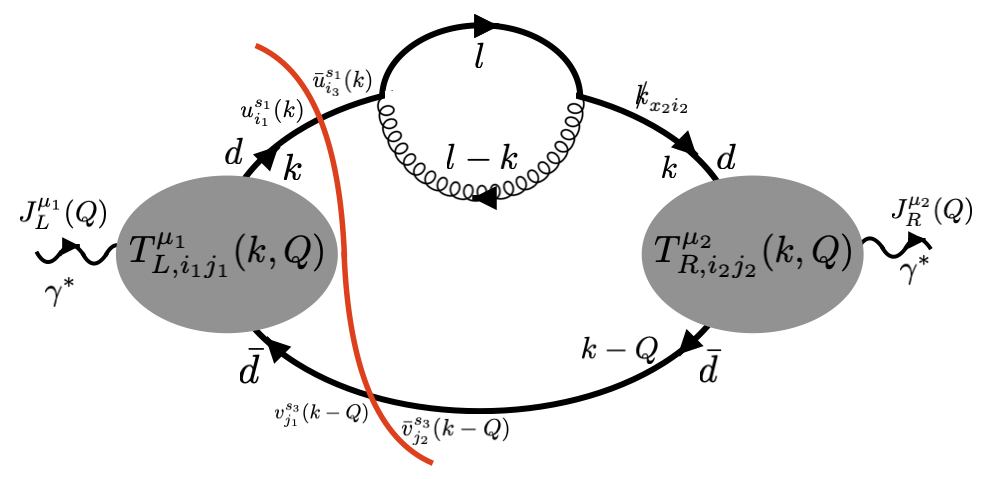
\includegraphics[width=1\linewidth]{CA.png}}
\end{minipage}\hfill
\begin{minipage}{0.5\linewidth}
\centering
{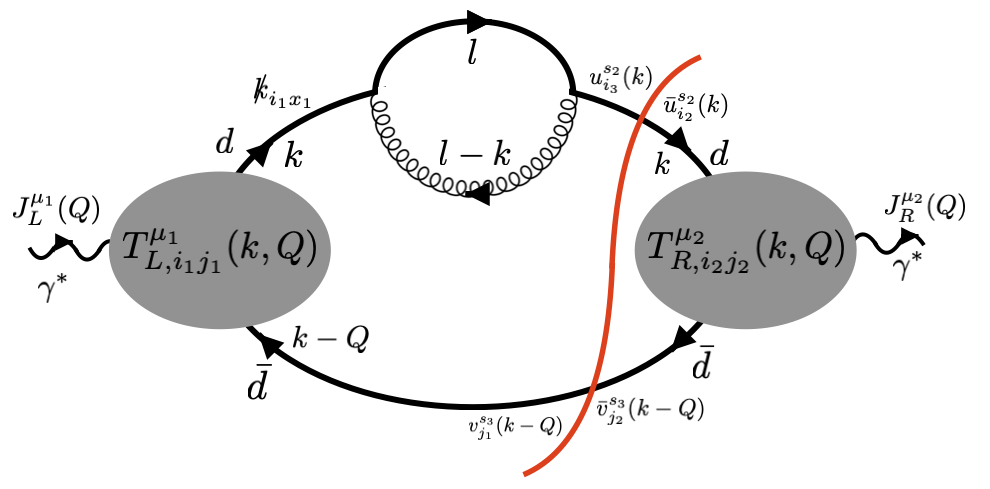
\includegraphics[width=1\linewidth]{CB.png}}
\end{minipage}
{\caption{\label{CAB} Cutkosky contributions C$_\textrm{A}$ (left) and C$_\textrm{B}$ (right).}}
\end{center}
\end{figure}
\noindent where each Cutkoski cut of a four-momentum $q$ translates into the expression $(-2\pi i)\delta^{+}\left(q^2\right)$.
We can now write explicitly the contributions C$_\textrm{A}$ and C$_\textrm{B}$ as:
\begin{eqnarray}
\label{CABdef}
{\textrm{C}}_{\textrm{A}}&=& (-2\pi i)^2 \delta^{+}\left((k-Q)^2\right)\delta^{+}\left(k^2\right)  \sum_{s_1 \in \pm} \sum_{s_3 \in \pm} 
\left( T^{L}_{i_1 j_1} v^{s_3}_{j_1} u^{s_1}_{i_1} \right )
\left( \bar{u}^{s_1}_{i_3} \Sigma^{R}_{i_3 x_2}(k,l) \frac{(-i)\slashed{k}_{x_2 i_2}}{k^2+i\delta} T^{R}_{i_2 j_2} \bar{v}^{s_3}_{j_2} \right) \nonumber\\
{\textrm{C}}_{\textrm{B}}&=& (-2\pi i)^2 \delta^{+}\left((k-Q)^2\right)\delta^{+}\left(k^2\right) \sum_{s_2 \in \pm} \sum_{s_3 \in \pm} 
\left( T^{L}_{i_1 j_1}  \frac{(i)\slashed{k}_{i_1 x_1}}{k^2-i\delta} \Sigma^{L}_{x_1 i_3}(k,l) u^{s_2}_{i_3} v^{s_3}_{j_1} \right )
\left( \bar{u}^{s_2}_{i_2}  T^{R}_{i_2 j_2} \bar{v}^{s_3}_{j_2} \right) \nonumber\\
\end{eqnarray}
with $T_{ij}\equiv J^\mu(k,Q) T^\mu_{ij}(k,Q)$ and where we kept implicit the dependences of the polarization vectors in the loop momenta.
The self-energy factors $\Sigma^{L/R}$ are defined as:
\begin{eqnarray}
\Gamma^{R}_{ij} (k) &\equiv& (-i) (\slashed{k}_{i j} ) + \left( \int \frac{\tilde{d}l}{(2\pi)^4} \Sigma^{R}_{ix} (k,l) \right)  (-i) (\slashed{k}_{x j} ) \nonumber\\
\Gamma^{L}_{ij} (k) &\equiv& (i) (\slashed{k}_{i j} ) + (i) (\slashed{k}_{i x} ) \left(\int \frac{\tilde{d}l}{(2\pi)^4} \Sigma^{L}_{x j}(k,l) \right)
\end{eqnarray}
where  $\int \tilde{d}l\; \equiv \left(\frac{\mu^2}{4\pi e^{-\gamma}}\right)^{\epsilon} \int \frac{d^{4-2\epsilon}l}{(2\pi)^{-2\epsilon}} $. When setting all couplings to 1, the explicit expressions of $\Sigma^{R/L}_{ij}$ then reads:
\begin{eqnarray}
\label{Fdefinitions}
B^R_{i_1 i_2}(k,l)&=& \left( \sum_{s_1 \in \pm} u^{s_1}_{i_1}(k) \bar{u}^{s_1}_{i_3}(k) \right) \Sigma^{R}_{i_3 x_2}(k,l)\frac{ (-i)\slashed{k}_{x_2 i_2}}{k^2-i\delta} \nonumber\\ 
&=& 2 C_F (1-\epsilon) [(i)(-i)(i)(i)](-i) \frac{ (-\slashed{k}\slashed{l}\slashed{k})_{i_3 i_2} }{(k^2-i\delta)(l^2-i\delta) ((l-k)^2-i\delta)} \nonumber\\
&=& 2 C_F (1-\epsilon) (-i) \frac{ (\slashed{k}\slashed{l}\slashed{k})_{i_1 i_2} }{(k^2-i\delta) (l^2-i\delta) ((l-k)^2-i\delta)} 
= 2 C_F (1-\epsilon) \mathcal{F}^R_{i_1i_2}(k,l))
\nonumber\\
B^L_{i_1 i_2}(k,l)&=& \frac{(i)\slashed{k}_{i_1 x_1}}{k^2+i\delta} \Sigma^{L}_{x_1 i_3}(k,l) \left( \sum_{s_2 \in \pm} u^{s_2}_{i_3}(k)\bar{u}^{s_2}_{i_2}(k)  \right) \nonumber\\
&=& 2 C_F (1-\epsilon) (i)[(-i)(i)(-i)(-i)] \frac{ (-\slashed{k}\slashed{l}\slashed{k})_{i_1 i_2} }{ (k^2+i\delta) (l^2+i\delta) ((l-k)^2+i\delta)}\nonumber\\
&=& 2 C_F (1-\epsilon) (i) \frac{ (\slashed{k}\slashed{l}\slashed{k})_{i_1 i_2} }{(k^2+i\delta) (l^2+i\delta) ((l-k)^2+i\delta)} 
= 2 C_F (1-\epsilon)  \mathcal{F}^L_{i_1i_2}(k,l)),
\nonumber \\  
\end{eqnarray}
where the $C_F$ terms comes from having performed the colour algebra.
Our target expression from eq.~\ref{CABdef} cannot be evaluated explicitly given that it is proportional to $\delta^{+}\left(k^2\right)/k^2$.
To address this issue, we will take advaxntage of the dispersion relation which we introduce in the next section.

\section{Dispersive representation}

Any function $f(x)$ and analytic in $\mathbb{C}\setminus(-\infty,-x^\star)\cup(x^\star,\infty)$ can be written using Cauchy's theorem by performing an integral along the contours indicated in fig.~\ref{IntegrationContours} below with $q^0\equiv x$ and $|\vec{q}|\equiv x^\star$:
\begin{figure}[ht!]
\begin{center}
\begin{minipage}{0.65\linewidth}
\centering
{\caption{\label{IntegrationContours} Integration contours considered for deriving the dispersion relation.}}
{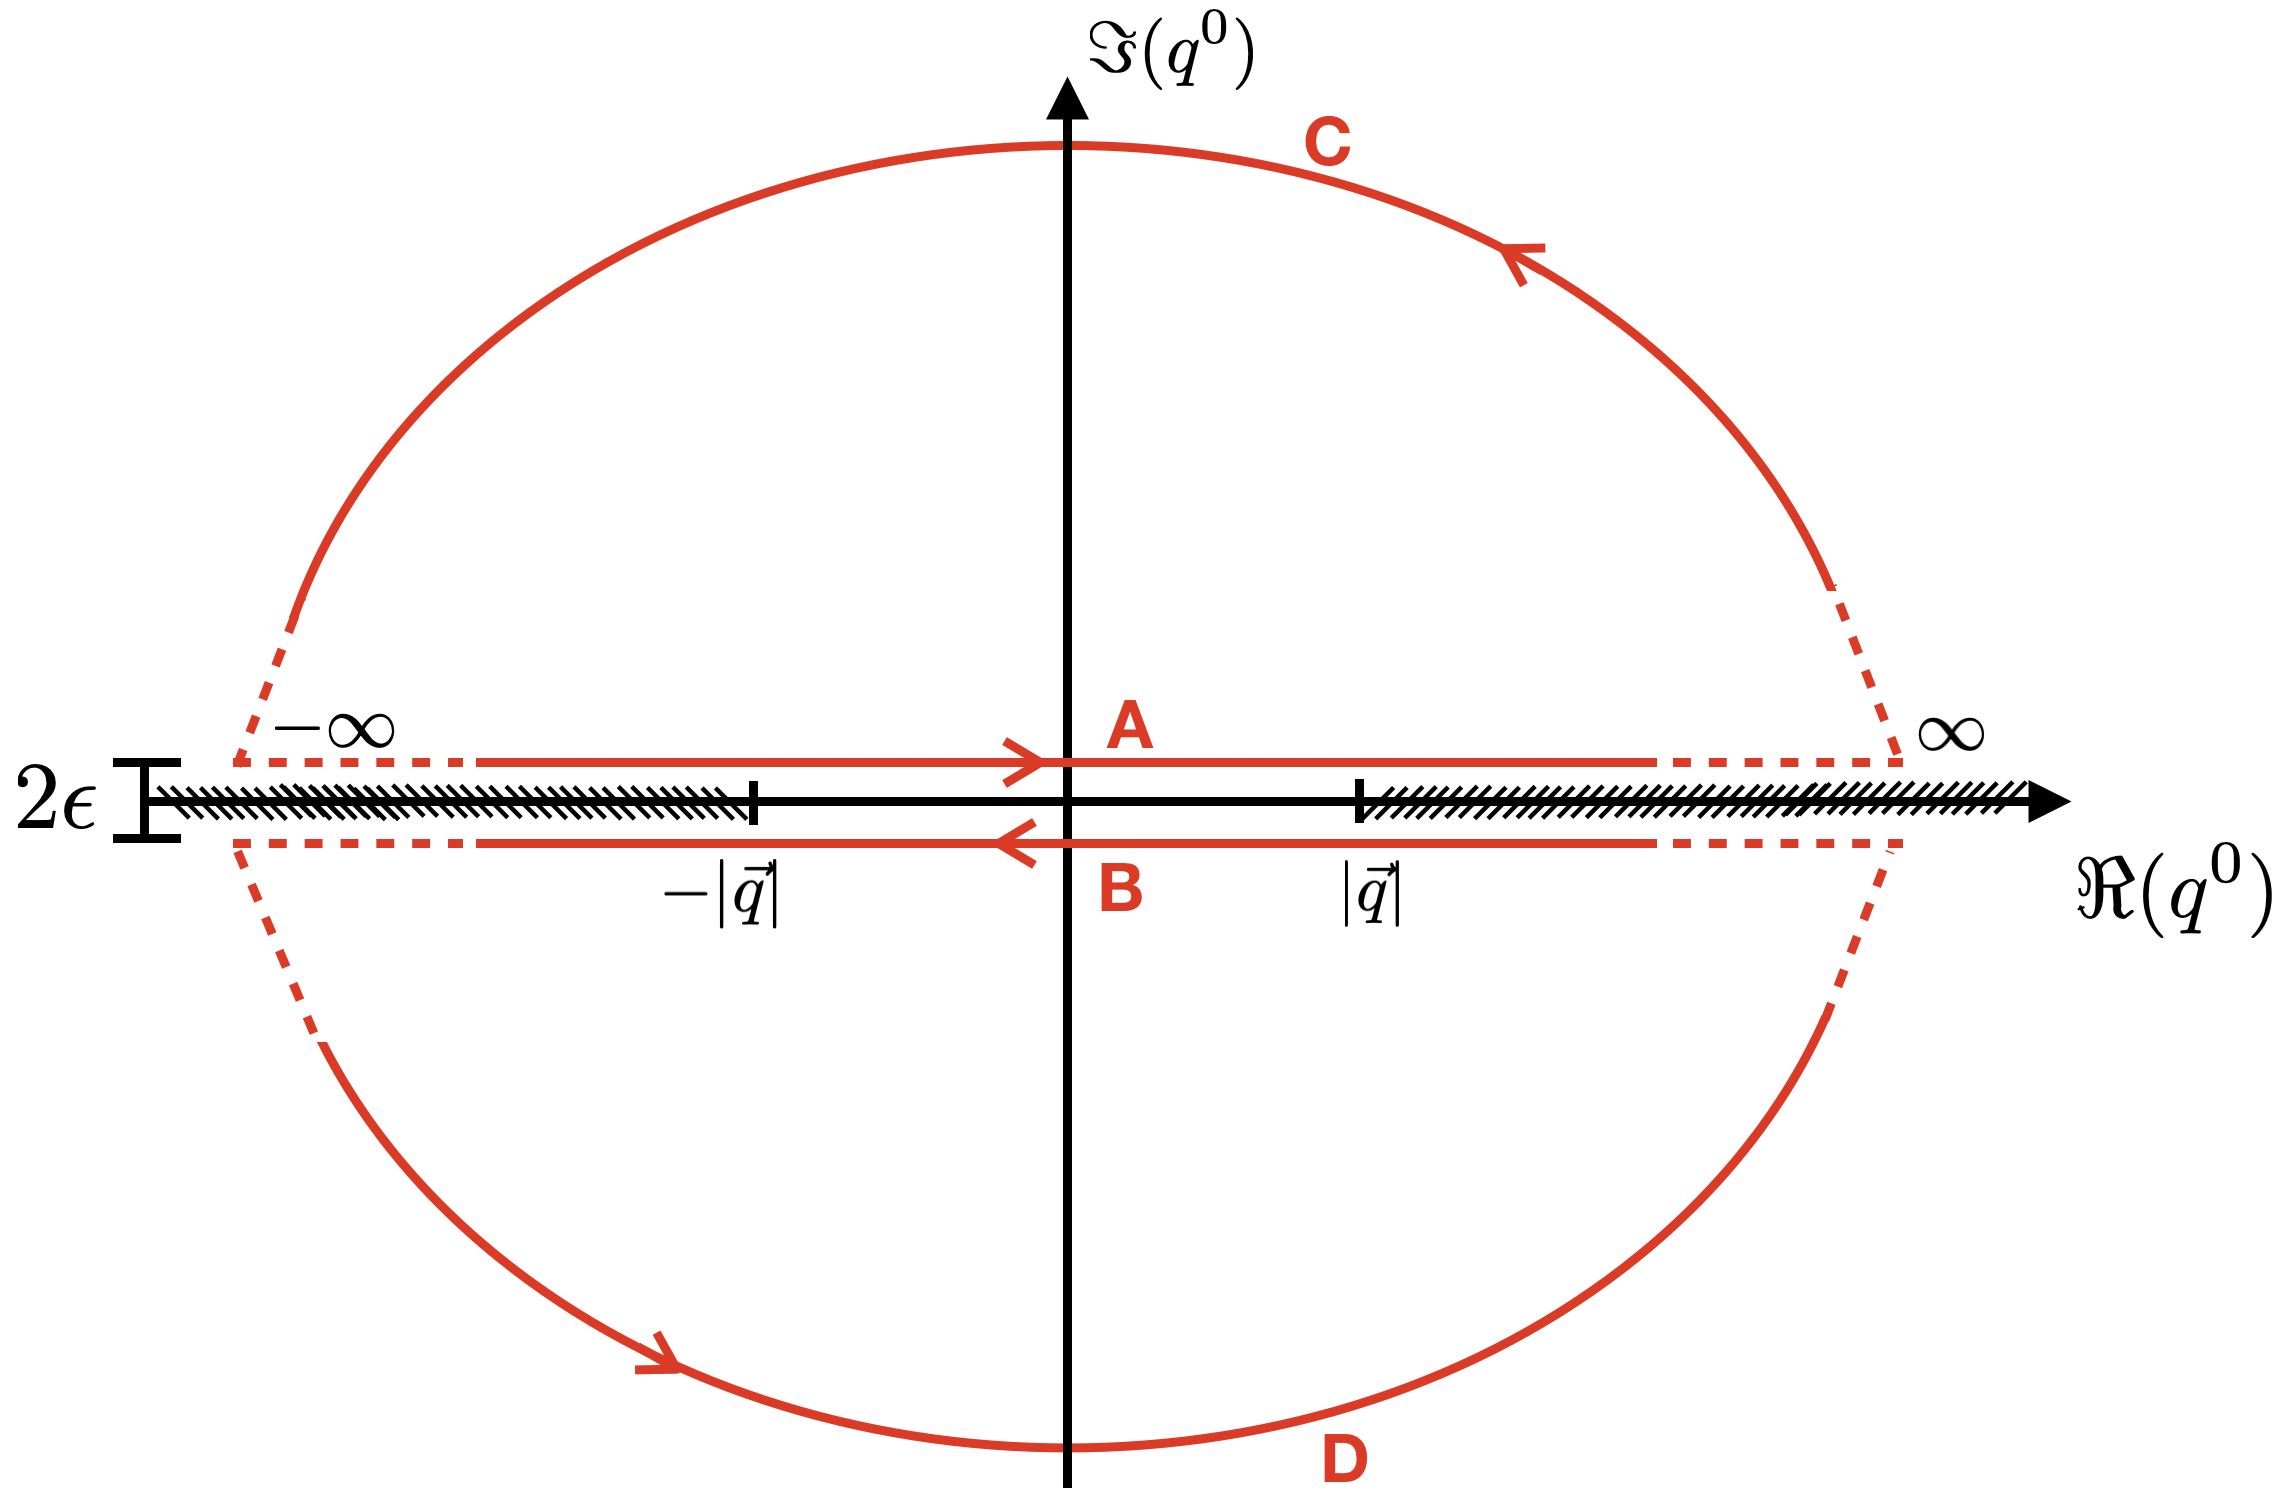
\includegraphics[width=0.75\linewidth]{integration_contour.png}}
\end{minipage}\hfill
\end{center}
\end{figure}
yielding the following dispersive expression for $f(x)$:
\begin{eqnarray}
f(x)&=& \lim_{\epsilon \rightarrow 0^+}\frac{1}{2\pi i} \left[ 
\underbrace{ \int_{-\infty}^\infty d z \frac{ f(z+i\epsilon) }{z-x+i\epsilon} }_{\textrm{segment A}} +
\underbrace{ \int_{\infty}^{-\infty} d z \frac{ f(z-i\epsilon) }{z-x-i\epsilon} }_{\textrm{segment B}}
\right ] \nonumber \\
&=& 
\frac{1}{2\pi i}  \lim_{\epsilon \rightarrow 0^+} \int_{-\infty}^\infty d z \frac{f(z+i\epsilon) - f(z-i\epsilon)   }{z-x} \nonumber \\
&=&
\frac{1}{2\pi i} \int_{-\infty}^\infty d z \frac{ \textrm{disc} \left[ f(z) \right] }{z-x}
=\frac{1}{2\pi i} \int_{0}^\infty d z \left[ \frac{ \textrm{disc} \left[ f(z) \right] }{z-x}-\frac{ \textrm{disc} \left[ f(-z) \right] }{z+x}\right]
,\label{DispertionRelation}
\end{eqnarray}
where we neglected the $\pm i \epsilon$ in the denominators of the second line because we assume that $f(s)$ is analytic everywhere except on $(-\infty,-x^\star)\cup(x^\star,\infty)$ which our contour never crosses. 
We also used the assumption\footnote{Notice that for this assumption to hold, it will be important that we include the denominator $\frac{1}{k^2}$ in the definition of $\mathcal{F}^{L/R}$ in eq.~\ref{Fdefinitions}. We stress that this property is then completely independent of whether or not one has performed UV renormalisation at this stage.} that $\lim_{|z| \rightarrow \infty} f(z) = 0$, allowing us to neglect the segments C and D of the contour at infinity. Finally, we find it useful to split the integration domain in the last line of eq.~\ref{DispertionRelation} so as to be able to integrate over only positive $z$ values.

We now consider applying eq.~\ref{DispertionRelation} to the particular case of both functions $\mathcal{F}^L_{i_1i_2}(k^0,\vec{k},l)$ and $\mathcal{F}^R_{i_1i_2}(k^0,\vec{k},l)$, and considering $x\equiv k^0$.
We will also take advantage of the fact that self-energy functions satisfy (at any order in perturbation theory and also for massive internal lines (?) ) the reality condition known as the \emph{Schwartz reflection principle}, namely:
\begin{equation}
\mathcal{F}^{L/R}_{i_1i_2}(z^*, \vec{k},l)=\mathcal{F}^{L/R}_{i_1i_2}(z, \vec{k},l)^*
\end{equation}
which allows us to rewrite the discontinuity as:
\begin{eqnarray}
\textrm{disc} \left[ \mathcal{F}^{L/R}_{i_1i_2}(z, \vec{k},l) \right] &=& \lim_{\epsilon->0^+} \left( \mathcal{F}^{L/R}_{i_1i_2}(z+i\epsilon, \vec{k},l) - \mathcal{F}^{L/R}_{i_1i_2}(z-i\epsilon, \vec{k},l) \right ) \nonumber \\
&=&  \lim_{\epsilon \rightarrow 0^+} \left( \mathcal{F}^{L/R}_{i_1i_2}(z+i\epsilon, \vec{k},l) - \mathcal{F}^{L/R}_{i_1i_2}(z+i\epsilon, \vec{k},l)^* \right )\nonumber \\
&=&  2 i \lim_{\epsilon \rightarrow 0^+}  \Im{ \left[ \mathcal{F}^{L/R}_{i_1i_2}(z+i\epsilon, \vec{k},l) \right] } \nonumber \\
&=&  i \sum_{\textrm{C}^+_i\in \mathcal{C}_\mathcal{F}^{L/R}} \textrm{C}^+_i\left[ \mathcal{F}^{L/R}_{i_1i_2}(z, \vec{k},l)\right ],
\label{DiscIntoCutkosky}
\end{eqnarray}
where $\mathcal{C}_\mathcal{F}^{L/R}$ denote the list of Cutkosky cuts the integral $\mathcal{F}^{L/R}$ is subject to while the application of the \emph{signed} Cutkosky operator $C^{\pm}_i$ appearing on the last line reads:
\begin{equation}
C^{\pm}_i = (\mp2\pi i)^{|\textrm{cuts}_i|} \prod_{j\in \textrm{cuts}_i} q_j^2(z) \delta^{\pm}\left(q_j^2(z)\right)
\end{equation}
({\bf WARNING:} at this stage it seems that the above Cutkosky rule should \emph{not} involve a complex conjugation on the expression of the graph sitting on the right-hand side of the cut!).
We note that the last equality in eq.~\ref{DiscIntoCutkosky} stems from the Cutkosky rule that expresses the discontinuity of loop integrals, as written in Eq. (55) of ref.~\cite{Zwicky:2016lka}.
Also, for a complete unknown reason {\bf{HELP HERE!}}, the discontinuity of $\mathcal{F}^{L}$ is only non-zero for \emph{positive} energy $k^0$ while $\mathcal{F}^{R}$ only contributes to the discontinuity at a \emph{negative} $k^0$.
We thus arrive at the following final expression for the re-expression of $\mathcal{F}^{L/R}$ as quantities we will denote $\mathcal{\tilde{F}}^{R}$ and that are computed through the dispersive relation:
\begin{eqnarray}
\label{dispertionRelationApplied}
\mathcal{\tilde{F}}^{L}_{i_1i_2}(k^0, \vec{k},l) = \frac{1}{2\pi} \int_{0}^\infty d z \frac{ \sum_{\textrm{C}^+_i\in\mathcal{C}_\mathcal{F}^{L}} \textrm{C}^+_i\left[ \mathcal{F}^{L}_{i_1i_2}(z, \vec{k},l)\right ] }{z-k^0} \nonumber\\
\mathcal{\tilde{F}}^{R}_{i_1i_2}(k^0, \vec{k},l) = -\frac{1}{2\pi} \int_{0}^\infty d z \frac{ \sum_{\textrm{C}^-_i\in\mathcal{C}_\mathcal{F}^{R}} \textrm{C}^-_i\left[ \mathcal{F}^{R}_{i_1i_2}(-z, \vec{k},l)\right ] }{z+k^0} \nonumber\\
\end{eqnarray} 
\emph{PS:} Ideally one should be able to ditch the "dispersive" representation and find a way to arrive at the same expressions starting from the two-loop vacuum diagram formed by the one-loop bubble with the external leg closed onto itself:
\begin{figure}[ht!]
\begin{center}
\begin{minipage}{0.75\linewidth}
\centering
{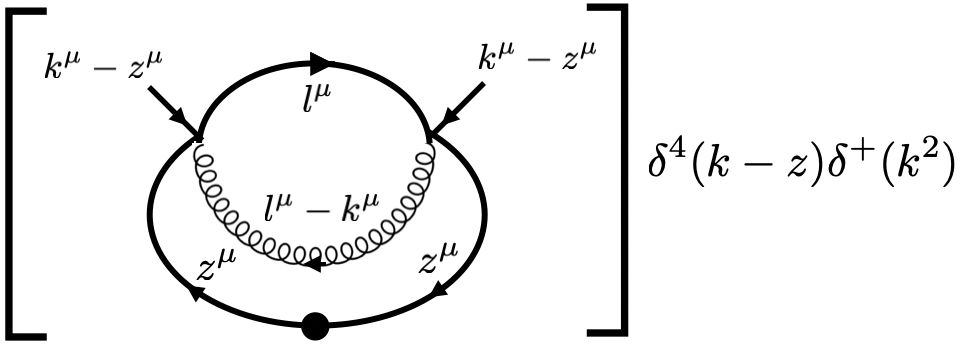
\includegraphics[width=1\linewidth]{LTD_instead_of_dispersive.png}}
\end{minipage}\hfill
{\caption{\label{DispersiveAlternative} Possible alternative representation of the dispersive representation that could be entirely derived within our LTD framework.}}
\end{center}
\end{figure}
Then maybe one could proceed like for normal two-loop LTD and finally impose $\delta^4(z-k)\delta(k^2)$ on the final expression, although it is not clear how to do so at this stage...
\section{Direct evaluation}

We now turn to directly evaluating the two expressions of Eq.~\ref{dispertionRelationApplied}. 
A first thing to note is that the set of cuts in $\mathcal{C}_\mathcal{F}^{L/R}$ are identical, except for their sign, in both the $L$ and $R$ contributions and it reads:
\begin{equation}
\mathcal{C}_\mathcal{F}^{L/R} \equiv \{ (2\pi i)^2 (l^2) (l-k)^2 \delta^{+/-}\left(l^2\right)\delta^{+/-}\left((l-k)^2\right)\}
\end{equation}
It is also worth noting that it is important that we do not consider further complex conjugation in the application of the Cutkosky operator above, as this would yield an extra incorrect minus sign in contribution $\textrm{C}_\textrm{B}$ of fig.~\ref{CAB}. The lack of complex conjugation in the application of these \emph{bubble Cutkosky cuts} also implies that the sign of the causal prescription involved in the contributions $\mathcal{F}^{L/R}_{i_1 i_2}$ remains unchanged!

It is useful at this stage to provide a graphical representation of the dispersion relation of eq.~\ref{dispertionRelationApplied} combined with the overall contributions ${\textrm{C}}_{\textrm{A}}$ and ${\textrm{C}}_{\textrm{B}}$ of fig.~\ref{CAB}:
\begin{figure}[ht!]
\begin{center}
\begin{minipage}{0.5\linewidth}
\centering
{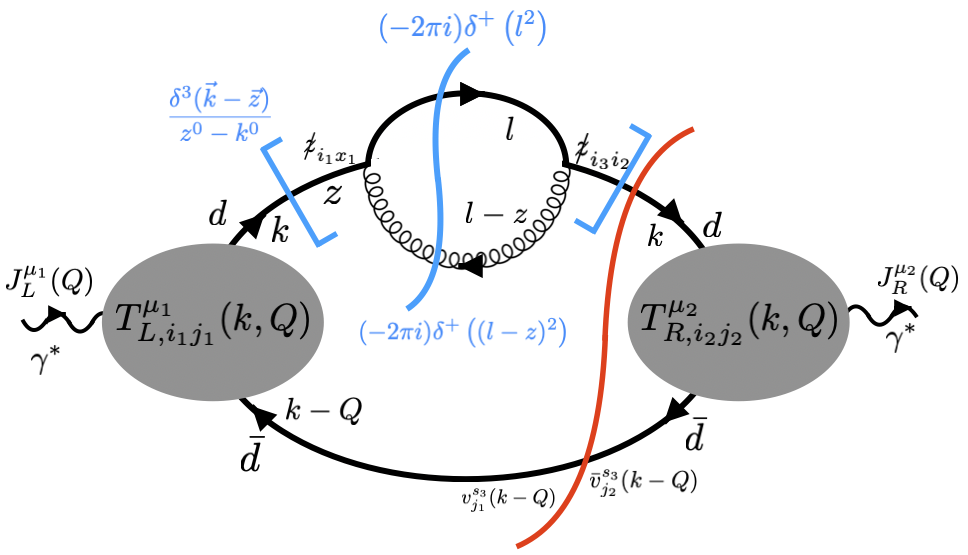
\includegraphics[width=1\linewidth]{CA_bubble_cut.png}}
\end{minipage}\hfill
\begin{minipage}{0.5\linewidth}
\centering
{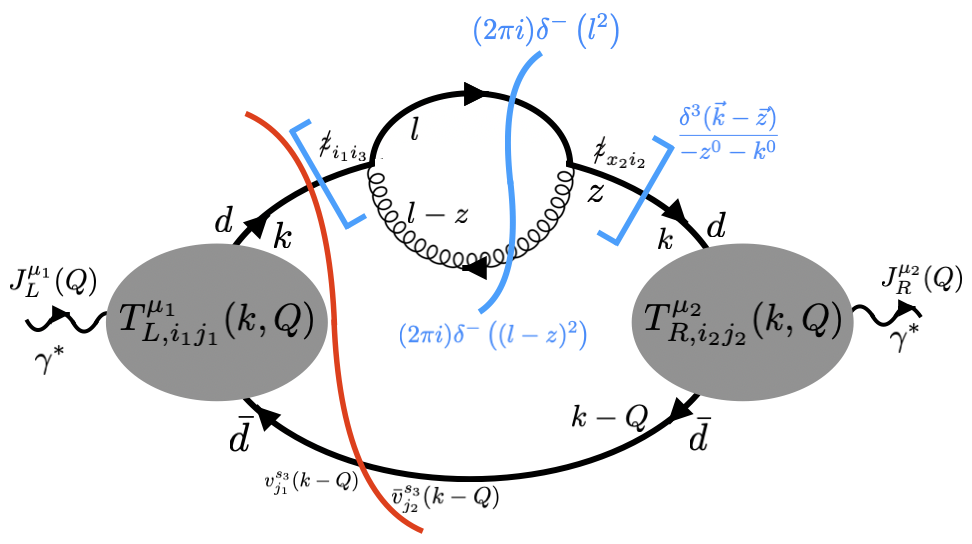
\includegraphics[width=1\linewidth]{CB_bubble_cut.png}}
\end{minipage}
{\caption{\label{CABwithBubbleCuts} Contributions C$_\textrm{A}$ (left) and C$_\textrm{B}$ (right), including bubble cuts (in blue) stemming from the dispersive representation of eq.~\ref{dispertionRelationApplied}. The squared blue cut indicate a break in the energy conservation between $z^\mu=(z,\vec{k})$ and $k^\mu=(k^0,\vec{k})$.}}
\end{center}
\end{figure}
Pay attention in particular how the polarization vectors $u_{i_1}^{s_1}(k)$ and $\bar{u}_{i_2}^{s_2}(k)$ have been pulled \emph{inside} the expression of the bubble subject to the dispersive representation. This implies that the momentum dependency in these polarisation vectors changes from $k$ to $z$, thus allowing us to simplify the polarisation sum into $\slashed{z}_{i_3 i_2}$ and $\slashed{z}_{i_1 i_3}$ respectively, as done in eq.~\ref{Fdefinitions}.

We are now ready to explicitly compute $\mathcal{\tilde{F}}^{L}_{i_1i_2}(k^0, \vec{k},l)$ as in eq.~\ref{dispertionRelationApplied}, while also pulling in the integration measure $\int \frac{\tilde{d} l}{(2\pi)^4}$ and swapping the order of integration with $\int d z$:
\begin{eqnarray}
\label{CBexplicit}
\textrm{C}_\textrm{B}\left(k \right) &=& \underbrace{T^{L}_{j_1 i_1} (\slashed{k}-\slashed{Q})_{j_2 j_1} T^{R}_{i_2 j_2} 2 C_F (1-\epsilon)  }_{T_{i_2 i_1}(k,Q,\epsilon)}  \int \frac{\tilde{d} l}{(2\pi)^4} \mathcal{\tilde{F}}^{L}_{i_1i_2}(k^0, \vec{k},l) \nonumber\\
&=&T_{i_2 i_1}  \int \frac{\tilde{d} l}{(2\pi)^4}  \frac{1}{2\pi} \int_{0}^\infty d z^0 \frac{ \sum_{\textrm{C}^+_i\in\mathcal{C}_\mathcal{F}^{L}} \textrm{C}^+_i\left[ \mathcal{F}^{L}_{i_1i_2}(z^0, \vec{k},l)\right ] }{z^0-k^0} \nonumber \\
&=&T_{i_2 i_1}  \int \frac{\tilde{d}^3 \vec{l}}{(2\pi)^4}  \frac{(-2\pi i)^2}{2\pi} \int_{0}^\infty d z^0 \frac{1}{z^0-k^0} \frac{(i)\slashed{z}\slashed{l}\slashed{z}}{z^2 (2 |\vec{l}|) (2 |\vec{l}-\vec{k}|)} \delta \left(z^0-|\vec{l}|-|\vec{l}-\vec{k}|\right), \nonumber \\
\end{eqnarray}
with $z\equiv(z^0,\vec{k})$.
For $\textrm{C}_\textrm{A}$ we get:
\begin{eqnarray}
\label{CAexplicit}
\textrm{C}_\textrm{A}\left(k \right) &=& T_{i_2 i_1} \int \frac{\tilde{d} l}{(2\pi)^4} \mathcal{\tilde{F}}^{R}_{i_1i_2}(k^0, \vec{k},l)\nonumber\\
&=&T_{i_2 i_1}  \int \frac{\tilde{d} l}{(2\pi)^4}  \frac{1}{2\pi} \int_{0}^\infty d z^0 \frac{ \sum_{\textrm{C}^-_i\in\mathcal{C}_\mathcal{F}^{R}} \textrm{C}^-_i\left[ \mathcal{F}^{R}_{i_1i_2}(-z^0, \vec{k},l)\right ] }{z^0-k^0} \nonumber \\
&=&T_{i_2 i_1}  \int \frac{\tilde{d}^3 \vec{l}}{(2\pi)^4}  \frac{(2\pi i)^2}{2\pi} \int_{0}^\infty d z^0 \frac{1}{-z^0-k^0} \frac{(-i)\slashed{\bar{z}}\slashed{\bar{l}}\slashed{\bar{z}}}{\bar{z}^2 (-2 |\vec{l}|) (-2 |\vec{l}-\vec{k}|)} \delta \left(-z^0+|\vec{l}|+|\vec{l}-\vec{k}|\right) \nonumber \\
\end{eqnarray}
with $\bar{z}\equiv(-z^0,\vec{k})$ and $\bar{l}\equiv(-l^0,\vec{l})$.
When combining $\textrm{C}_\textrm{A}$ and $\textrm{C}_\textrm{B}$ we find:
\begin{eqnarray}
\textrm{C}_\textrm{B}+ \textrm{C}_\textrm{A} &=& (-i)T_{i_2 i_1}  \int \frac{\tilde{d}^3 \vec{l}}{(2\pi)^3} \int_{0}^\infty d z^0 \frac{\delta \left(z^0-|\vec{l}|-|\vec{l}-\vec{k}|\right)}{(z^0)^2-(k^0)^2} \frac{1}{(2 |\vec{l}|) (2 |\vec{l}-\vec{k}|)} \nonumber \\
&\times&\left( 
\frac{z^0+k^0}{z^2} \slashed{z}\slashed{l}\slashed{z} + \frac{z^0-k^0}{\bar{z}^2} \slashed{\bar{z}}\slashed{\bar{l}}\slashed{\bar{z}}
\right)
\end{eqnarray}
Since $z^2=\bar{z}^2$ 
% and also that:
%\begin{eqnarray}
%\slashed{\bar{z}}\slashed{\bar{l}}\slashed{\bar{z}}&=&(-z^0\gamma^0+\vec{k} \cdot \vec{\gamma}) \slashed{l} (-z^0\gamma^0+\vec{k} \cdot \vec{\gamma}) \nonumber\\
%&=&\slashed{z}\slashed{l}\slashed{z}- 2 z^0\left( \gamma^0 \slashed{l} (\vec{k} \cdot \vec{\gamma}) + (\vec{k} \cdot \vec{\gamma}) \slashed{l} \gamma^0 \right) \nonumber\\
%&=&-\slashed{z}\slashed{l}\slashed{z} + 2 (z^0)^2 \gamma^0 \slashed{l} \gamma^0 + 2 (\vec{k} \cdot \vec{\gamma}) \slashed{l} (\vec{k} \cdot \vec{\gamma}),
%\end{eqnarray}
we write the final expression for $\textrm{C}_\textrm{B}+ \textrm{C}_\textrm{A}$ by performing the integration over $z^0$ with $\delta \left(z^0-|\vec{l}|-|\vec{l}-\vec{k}|\right)$ and introducing the variable $z^\star \equiv |\vec{l}|+|\vec{l}-\vec{k}|$:
%\begin{eqnarray}
%\label{OurFinalOffshellExpressionSelfEnergy}
%&& \textrm{C}_\textrm{B}+ \textrm{C}_\textrm{A} = (-i)T_{i_2 i_1}  \nonumber\\
%&& \times \int \frac{\tilde{d}^3 \vec{l}}{(2\pi)^3}
%\frac{
%z^\star \left( 2 (z^\star)^2 \gamma^0 \slashed{l} \gamma^0 + 2 (\vec{k} \cdot \vec{\gamma}) \slashed{l} (\vec{k} \cdot \vec{\gamma}) \right) +
%k^0 \left (
%2 z^\star\left( \gamma^0 \slashed{l} (\vec{k} \cdot \vec{\gamma}) + (\vec{k} \cdot \vec{\gamma}) \slashed{l} \gamma^0 \right)
%\right) 
%}{
%\left( (z^\star)^2-(k^0)^2 \right) \left( (z^\star)^2-|\vec{k}|^2\right) \left( 2 |\vec{l}|\; 2 |\vec{l}-\vec{k}| \right) } \nonumber\\
%\end{eqnarray}
\begin{eqnarray}
\label{OurFinalOffshellExpressionSelfEnergy}
&& \textrm{C}_\textrm{B}+ \textrm{C}_\textrm{A} = (-i)T_{i_2 i_1} \int \frac{\tilde{d}^3 \vec{l}}{(2\pi)^3}
\frac{
(z^\star+k^0) \slashed{z}\slashed{l}\slashed{z} + (z^\star-k^0)  \slashed{\bar{z}}\slashed{\bar{l}}\slashed{\bar{z}}
}{
\left( (z^\star)^2-(k^0)^2 \right) \left( (z^\star)^2-|\vec{k}|^2\right) \left( 2 |\vec{l}|\; 2 |\vec{l}-\vec{k}| \right) } \nonumber\\
\end{eqnarray}
When considering the case of an external bubble (as in fig.~\ref{CABwithBubbleCuts}), we can pull in the Cutkosky cut $(-2\pi i)\delta^2\left(k^2\right)$ which simplifies the above a bit as follows:
%\begin{eqnarray}
%\label{OurFinalExpressionSelfEnergy}
%&& \left( \textrm{C}_\textrm{B}+ \textrm{C}_\textrm{A}\right) (-2\pi i)\delta^2\left(k^2\right) = \frac{(-2\pi i)}{2|\vec{k}|}(-i)T_{i_2 i_1}  \nonumber\\
%&& \times \int \frac{\tilde{d}^3 \vec{l}}{(2\pi)^3}
%\frac{
%z^\star \left( 2 (z^\star)^2 \gamma^0 \slashed{l} \gamma^0 + 2 (\vec{k} \cdot \vec{\gamma}) \slashed{l} (\vec{k} \cdot \vec{\gamma}) \right) +
%|\vec{k}| \left (
%2 z^\star\left( \gamma^0 \slashed{l} (\vec{k} \cdot \vec{\gamma}) + (\vec{k} \cdot \vec{\gamma}) \slashed{l} \gamma^0 \right)
%\right) 
%}{
%\left( (z^\star)^2-|\vec{k}|^2\right)^2 \left( 2 |\vec{l}|\; 2 |\vec{l}-\vec{k}| \right) }. \nonumber\\
%\end{eqnarray}
\begin{eqnarray}
\label{OurFinalExpressionSelfEnergy}
&& \left( \textrm{C}_\textrm{B}+ \textrm{C}_\textrm{A}\right) (-2\pi i)\delta^2\left(k^2\right) = \frac{(-2\pi i)}{2|\vec{k}|}(-i)T_{i_2 i_1}  \int \frac{\tilde{d}^3 \vec{l}}{(2\pi)^3}
\frac{
(z^\star+|\vec{k}|) \slashed{z}\slashed{l}\slashed{z} + (z^\star-|\vec{k}|)  \slashed{\bar{z}}\slashed{\bar{l}}\slashed{\bar{z}}
}{
\left( (z^\star)^2-|\vec{k}|^2\right)^2 \left( 2 |\vec{l}|\; 2 |\vec{l}-\vec{k}| \right) } \nonumber\\
\end{eqnarray}
As we can see, the above expression of the quark self-energy is not as elegant as eq.(336) of Soper's Beowulf notes, because we did not choose a smart momentum routing allowing him to perform the Lorentz algebra shown in his eq.(331).
This implies that we could not explicitly cancel the $\left( (z^\star)^2-|\vec{k}|^2\right)$ denominator in eq.~\ref{OurFinalOffshellExpressionSelfEnergy} (which is not formally necessary, for example Soper also does not cancel it in the case of the self-energy of the gluon). 
However, our expression of eq.~\ref{OurFinalExpressionSelfEnergy} is formally equivalent to Soper's one, as explicitly shown in the Mathematica notebook accompanying these notes.

The expression of eq.~\ref{OurFinalExpressionSelfEnergy} has a superficial degree of UV divergence in $|\vec{l}|$ of $7-6=1$ (as in Soper's case) which therefore calls for local UV counterterms cancelling both the leading \emph{and subleading} UV behaviour and reproducing the on-shell renormalisation conditions of eqs.~\ref{renormConditionsA}-\ref{renormConditionsD}.
This is the object of the next section. 

\section{UV local counterterms}

In this section, we aim at designing local UV counterterms for the contributions $\mathcal{\tilde{F}}^{L}_{i_1i_2}(k^0, \vec{k},l)$ and $\mathcal{\tilde{F}}^{R}_{i_1i_2}(k^0, \vec{k},l)$.
We will denote these counterterms $\mathcal{\bar{F}}^{L}_{i_1i_2}(k^0, \vec{k},l)$ and $\mathcal{\bar{F}}^{R}_{i_1i_2}(k^0, \vec{k},l)$ respectively and they must be designed so as satisfy the following properties (remember that $\slashed{k}\slashed{k}=k^2$):
\begin{itemize}
\item C1) $\lim_{|\vec{l}|\rightarrow \infty} |\vec{l}|^3 \left[ \mathcal{\tilde{F}}^{L/R}_{i_1i_2}(k^0, \vec{k},l) - \mathcal{\bar{F}}^{L/R}_{i_1i_2}(k^0, \vec{k},l) \right] =0$
\item C2) $\lim_{k^0\rightarrow |\vec{k}|} \slashed{k} \int \tilde{d}l \left[ \mathcal{\tilde{F}}^{L}_{i_1i_2}(k^0, \vec{k},l) - \mathcal{\bar{F}}^{L}_{i_1i_2}(k^0, \vec{k},l) \right] =0$ (from eq.~\ref{renormConditionsA})
\item C3) $\lim_{k^0\rightarrow |\vec{k}|} \int \tilde{d}\;l \left[ \mathcal{\tilde{F}}^{R}_{i_1i_2}(k^0, \vec{k},l) - \mathcal{\bar{F}}^{R}_{i_1i_2}(k^0, \vec{k},l) \right] \slashed{k} =0$ (from eq.~\ref{renormConditionsB})
\item C4) $\lim_{k^0\rightarrow |\vec{k}|} \int \tilde{d} \left[ \mathcal{\tilde{F}}^{L}_{i_1i_2}(k^0, \vec{k},l) - \mathcal{\bar{F}}^{L}_{i_1i_2}(k^0, \vec{k},l) \right] =0$ (directly from eq.~\ref{renormConditionsC})
\item C5) $\lim_{k^0\rightarrow |\vec{k}|} \int \tilde{d} \left[ \mathcal{\tilde{F}}^{R}_{i_1i_2}(k^0, \vec{k},l) - \mathcal{\bar{F}}^{R}_{i_1i_2}(k^0, \vec{k},l) \right] =0$ (directly from eq.~\ref{renormConditionsD})
\end{itemize}
We already see here an apparent difference w.r.t Soper's approach where he insists on enforcing the following on his UV counterterm:
\begin{equation}
\lim_{k^0\rightarrow |\vec{k}|} \int \tilde{d}l \mathcal{\bar{F}}^{L/R}_{i_1i_2}(k^0, \vec{k},l) = 0,
\end{equation}
which would correspond to the $\overline{\textrm{MS}}$ renormalisation conditions (as he claims himself) which I believe are not appropriate in the context of the renormalisation of external self-energies. But it may be that this makes not difference in the case of massless quarks since we know that their wavefunction UV counterterms have no finite piece \emph{also} in the on-shell scheme. This would however definitely make a difference for massive quarks (a.k.a top-quark).

In order to separate the task of satisfying condition C1) and that of satisfying eqs. C2)$\rightarrow$C5), we will write our counterterms as:
\begin{equation}
\mathcal{\bar{F}}^{L/R}_{i_1i_2} = \mathcal{\hat{F}}^{L/R}_{i_1i_2}+\Delta \mathcal{\bar{F}}^{L/R}_{i_1i_2},
\end{equation}
where
\begin{eqnarray}
&&\lim_{|\vec{l}|\rightarrow \infty} |\vec{l}|^3 \Delta \mathcal{\bar{F}}^{L/R}_{i_1i_2}(k^0, \vec{k},l) = 0 \\
&&\lim_{k^0\rightarrow |\vec{k}|} \int \tilde{d} \Delta \mathcal{\bar{F}}^{L/R}_{i_1i_2}(k^0, \vec{k},l) = 
\lim_{k^0\rightarrow |\vec{k}|} \int \tilde{d} \left[ \mathcal{\tilde{F}}^{L/R}_{i_1i_2}(k^0, \vec{k},l) - \mathcal{\hat{F}}^{L/R}_{i_1i_2}(k^0, \vec{k},l) \right]. \label{constraintOnDeltaF}
\end{eqnarray}
In other terms, the role of $\mathcal{\hat{F}}^{L/R}_{i_1i_2}$ is to guarantee on its own that C1) is satisfied while the role of $\Delta \mathcal{\bar{F}}^{L/R}_{i_1i_2}$ is \emph{only} to insure that eqs. C2)$\rightarrow$C5) are satisfied.\\

In this section, we will focus only on designing $\mathcal{\hat{F}}^{L/R}_{i_1i_2}$.
We first note that it would be simple to design such counterterm if we could start from a clear four-dimensional picture similar to that of Fig.~\ref{DispersiveAlternative}.
Unfortunately, our current understanding of the relation between LTD and the dispersive formula does not allow us to do this and we must start from the last line of eq.~\ref{CBexplicit}, where the integration over $l^0$ has already be performed.
Within the dispersive approach we can only consider the UV behaviour *after* this energy integration as otherwise the UV divergence due to the apparition of $z^0$ in the denominator would not be manifest.
Our starting expression to approximate is therefore:
\begin{equation}
\textrm{C}_\textrm{B}\left(k \right) =
T_{i_2 i_1}  \int \frac{\tilde{d}^3 \vec{l}}{(2\pi)^3} (-i) \frac{1}{z^\star-k^0} \frac{\slashed{z}\slashed{l}\slashed{z}}{z^2 (2 |\vec{l}|) (2 |\vec{l}-\vec{k}|)},
\end{equation}
with $z^\star = |\vec{l}|+|\vec{l}-\vec{k}|$ and $z=(z^\star,\vec{k})$. Since the integrand goes like $|\vec{l}|^{-2}$ we will need to subtract \emph{both} the leading and subleading UV limit for condition C1) to be satisfied.
The brute force way to proceed is to write $\vec{l}=t\;\vec{\hat{l}}$ thus obtaining:
\begin{eqnarray}
 |\vec{l}|&=&t\sqrt{\hat{\vec{l}} \cdot  \hat{\vec{l}}} \\
 |\vec{l}-\vec{k}|&=&\sqrt{t^2\; \hat{\vec{l}} \cdot  \hat{\vec{l}}-t\; 2\hat{\vec{l}} \cdot \vec{k} + \vec{k} \cdot \vec{k}}.
 \end{eqnarray}
We can then expand the resulting expression in $t$ and retain all terms up to (and including) $\mathcal{O}(t^{-3})$.
Even though this would certainly be a valid candidate for $\mathcal{\hat{F}}^{L/R}_{i_1i_2}$, it is not clear how it relates to the one obtained by Soper and also whether we could easily accommodate the resulting denominators as "normal propagators" fitting our Rust implementation of the bubble problem.

\section{Matching renormalisation conditions}
In this section, we carry out the computing of the quantities $\Delta \mathcal{\bar{F}}^{L/R}_{i_1i_2}$.\\

{\bf{TODO: In principle this should "simply" amount to integrating eq.~\ref{constraintOnDeltaF} in dimensional regularisation and reverse-engineering a local expression integrating to that quantity... I don't see a systematic way of doing this however. Maybe contact Soper on the matter...
We should of course not forget however that we can always decide to add the integrated contribution of $\Delta \mathcal{\bar{F}}^{L/R}_{i_1i_2}$ through an additional form-factor of the lower-order super graph.
}}

\bibliographystyle{JHEP}
\bibliography{biblio}

\end{document}
